% DOC SETTINGS ===================================
\documentclass{article}
\usepackage[utf8]{inputenc}
\usepackage{steinmetz}
\usepackage{mathtools}  
\usepackage{multicol}
\usepackage{circuitikz}
\usepackage{listings}
\usepackage{geometry}
\usepackage{fancyhdr}
\pagestyle{fancy}
\lhead{ECE2214 Lab Report 4}
\rhead{Kavin Thirukonda 2021}
\fancyheadoffset{0mm}
 \geometry{
 a4paper,
 total={170mm,257mm},
 left=20mm,
 top=25mm,
 }
\mathtoolsset{showonlyrefs} 
\cfoot{}
% DOC SETTINGS ===================================
\begin{document}
\begin{enumerate}
    \item Calculations
    \begin{enumerate}
        \item  Calculations of physical parameters related to the transmission line and load G', L', C', $Z_0$ \& $Z_L$ for \textit{f} = 500MHz.
        \begin{align}
            G' \cong \frac{2\pi\sigma_s}{\ln(b/a)} = \boxed{200 \mu S/m}
        \end{align}
        \begin{align}
            L' \cong \frac{\mu_0\ln(b/a)}{2\pi}= \boxed{370 nH/m}
        \end{align}
        \begin{align}
            C' \cong \frac{2\pi\epsilon_s}{\ln(b/a)}= \boxed{67.7 pF/m}
        \end{align}
        \begin{align}
            R' \cong \boxed{0 \Omega/m}
        \end{align}
        \begin{align}
            Z_0 \cong \sqrt{\frac{L'}{C'}} = \boxed{74\Omega}
        \end{align}
        \begin{align}
            Z_L \cong \boxed{76.5+j48.2}
        \end{align}
        \item Calculations of associated wave equations parameters:$\alpha, \beta, \Gamma,$ and SWR for \textit{f} = 500MHz.
        \begin{equation}
            \gamma = j\omega\sqrt{L'C'} = j(2\pi\cdot500\cdot10^6)\sqrt{(370 nH/m)(67.7 pF/m)} = 0 + j15.723
        \end{equation}
        \begin{equation}
            \alpha = \boxed{0}
        \end{equation}
        \begin{equation}
            \beta = \boxed{j15.723}
        \end{equation}
        \begin{equation}
            \Gamma = \frac{Z_L-Z_0}{Z_L+Z_0} = \frac{2.5+j48.2}{150.5+j48.2} = \boxed{0.10809 +j0.28564}
        \end{equation}
        \begin{equation}
            \text{SWR} = \boxed{1.87938}
        \end{equation}
    \end{enumerate}
    \item Standing wave plots
    \begin{enumerate}
        \item 3 Plots of $\Tilde{|V(z)|}$ and $\Tilde{|I(z)|}$ with respect to position z for: t = 0, t = T/4, and t = T/2 (3 plots, 2 curves on each plots). 
        \begin{center}
            \boxed{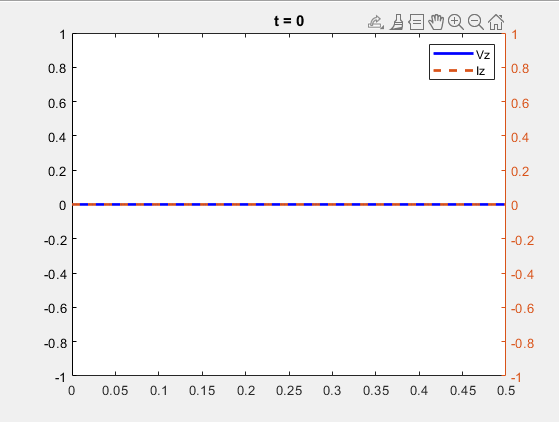
\includegraphics[width = .35\textwidth]{2a1.png}}
            \boxed{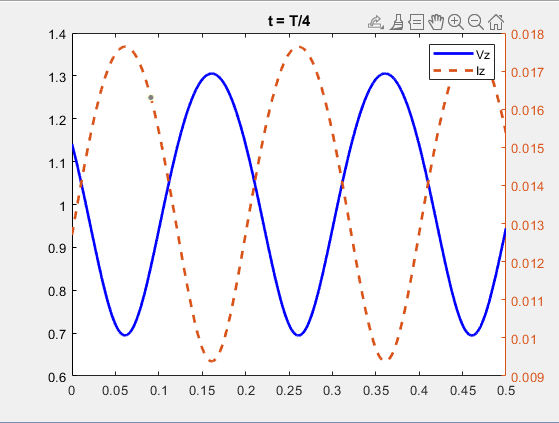
\includegraphics[width = .35\textwidth]{2a2.png}}
            \boxed{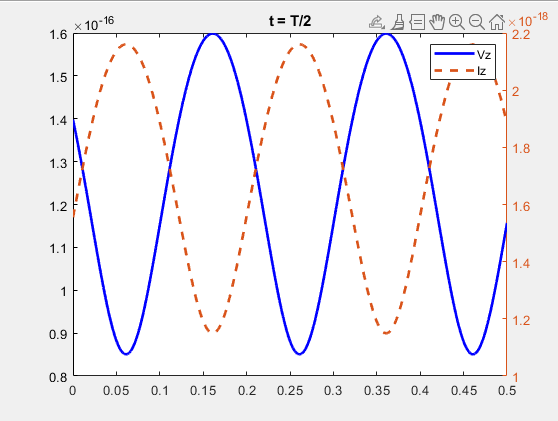
\includegraphics[width = .35\textwidth]{2a3.png}}
        \end{center}
        \item Plot of the voltage and current for $0 < t < 2T$ at z = d/2 (1 plot, 2 curves).
        \begin{center}
            \boxed{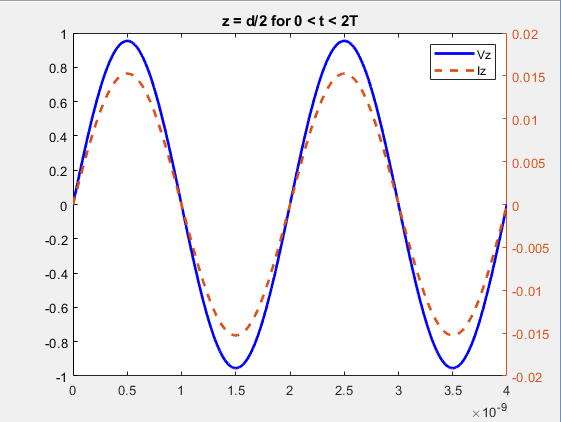
\includegraphics[width = .43\textwidth]{2b.png}}
        \end{center}
    \end{enumerate}
    \item Single-reactance matching
    \begin{enumerate}
        \item MATLAB numerical solving for the smallest positive $l_s$ and matching series reactance $X_s$ for \textit{f} = 500MHz
        \begin{equation}
            l_s = 0.10214703605560054313134437005654
        \end{equation}
        \begin{equation}
            X_s = -30.764510215082602
        \end{equation}
        \item MATLAB numerical solving for the smallest positive $l_p$ and matching series reactance $B_p$ for \textit{f} = 500MHz
        \begin{equation}
            l_p = 0.11767693593939264994013594545773
        \end{equation}
        \begin{equation}
            B_p = 0.008314732490563
        \end{equation}
        \item Plot of the reflection coefficient magnitude $|\Gamma|$ (between the source and transmission line) versus frequency \textit{f} from 50 MHz to 1 GHz (with increments of 50MHz or smaller)(2 plots, 1 curve on each plot).
        \begin{center}
            \boxed{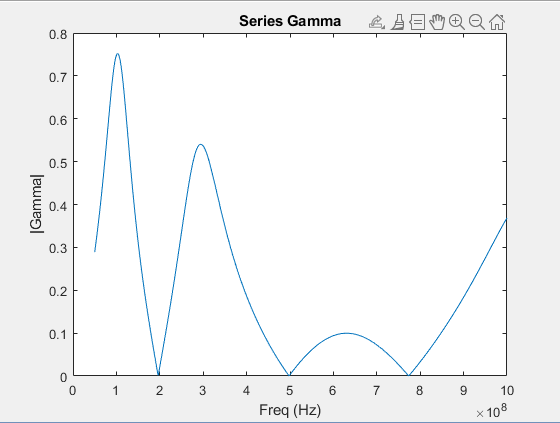
\includegraphics[width = .43\textwidth]{3c1.png}}
            \boxed{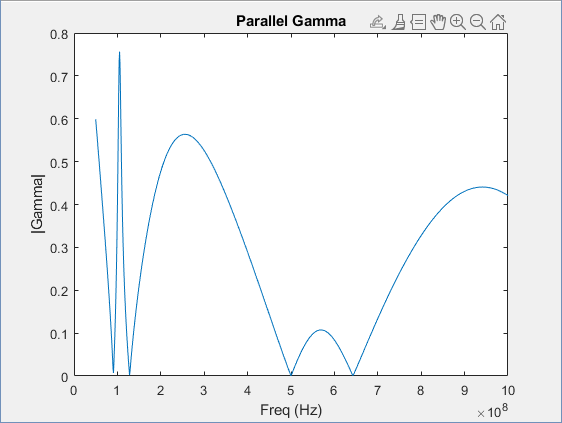
\includegraphics[width = .43\textwidth]{3c2.png}}
        \end{center}
        \item Measure the matching bandwidth with requirement $\Gamma \leq 0.3$ (between the source and transmission line), for each of the series and parallel configurations. Which configuration is better and why? 
        \begin{center}
            The \textbf{series} configuration is the best because it best fits the criteria given and sticks to the proper bounds.
        \end{center}
    \end{enumerate}
\end{enumerate}
\end{document}
